\documentclass[final]{article}

\usepackage{arxiv}

\usepackage[utf8]{inputenc} % allow utf-8 input
\usepackage[T1]{fontenc}    % use 8-bit T1 fonts
\usepackage{hyperref}       % hyperlinks
\usepackage{url}            % simple URL typesetting
\usepackage{booktabs}       % professional-quality tables
\usepackage{amsfonts}       % blackboard math symbols
\usepackage{nicefrac}       % compact symbols for 1/2, etc.
\usepackage{microtype}      % microtypography
\usepackage{lipsum}		% Can be removed after putting your text content
\usepackage{graphicx}
\usepackage{natbib}
\usepackage{doi}

\title{Fakenews Project}

%\date{September 9, 1985}	% Here you can change the date presented in the paper title
%\date{} 					% Or removing it

\author{ \hspace{1mm}Kristian Dam Pedersen\\
    tgz790\\
	%% examples of more authors
	\And
	Joshua Niemelä\\
    gmw103\\
	 \AND
	Jákup Lützen\\
    qkz344\\
	%% Affiliation \\
	%% Address \\
	%% \texttt{email} \\
	%% \And
	%% Coauthor \\
	%% Affiliation \\
	%% Address \\
	%% \texttt{email} \\
	%% \And
	%% Coauthor \\
	%% Affiliation \\
	%% Address \\
	%% \texttt{email} \\
}

% Uncomment to remove the date
%\date{}

% Uncomment to override  the `A preprint' in the header
\renewcommand{\headeright}{Technical Report}
%\renewcommand{\undertitle}{Technical Report}
%\renewcommand{\shorttitle}{\textit{arXiv} Template}

%%% Add PDF metadata to help others organize their library
%%% Once the PDF is generated, you can check the metadata with
%%% $ pdfinfo template.pdf
\hypersetup{
pdftitle={A template for the arxiv style},
pdfsubject={q-bio.NC, q-bio.QM},
pdfauthor={David S.~Hippocampus, Elias D.~Striatum},
pdfkeywords={First keyword, Second keyword, More},
}


\begin{document}
\maketitle
\graphicspath{{./src/}}
% keywords can be removed
%\keywords{First keyword \and Second keyword \and More}

\section*{Introduction}
Fake news has increasingly entered the public discourse in recent years. The Oxford English Dictionary coined the term
in 2013, and since then the use of the term has only gotten more and more common. We've encountered
novel challenges with regards to the spreading of false information, both through informal means (such as social media)
and increasingly through traditional media as well. In this technical report, we'll throw our hat
into the ring, by building a fake news classifier using 3 different complex models (a large deep neural network, a
smaller DNN and a model based on XGBoost). We'll start by going over our
data cleaning and processing. We will then use logistic regression to create a simple model that we can use as a
baseline. We will then go over our choice of complex models, before we take a look at the results and compare
performance across the different models. We will also evaluate our models on a novel dataset (LIAR), to assess wether
they generalise to unfamiliar domains.


\section{Data Exploration}

\subsection{Importing the FakeNewsCorpus dataset.}
The first challenge was simply downloading and unpacking the files on our Linux systems. We ended up concatenating the
files into a temporary zip file using \texttt{cat} and then unzipping the file using \texttt{unzip}. \\

Trying to read the data in python proved to be a challenging task, as the .csv file seemed to be corrupted or malformed
with rows containing different amounts of columns. Some article content included \texttt{\textbackslash r} (a carriage
return), which was interpreted as "newline", and thus, a new row in the middle of arbitrary news content. A single command '\texttt{sed 's/\textbackslash r/ /g' in.csv > out.csv}' replacing the carriage returns with spaces (to preserve word boundaries) turned out to solve this issue, and allowed us to use the entire dataset.\\
% \todo{Perhaps missing a section on summary statistics?}

\subsection{Larger than memory datasets}
Due to the size of our dataset, we had to use different methods for handling our data. Throughout this report we used 3
different methods: SQL Databases, chunk-wise streaming and brute force (access
to a large enough server). After getting the data into a readable CSV file in the previous step, we decided to load it
into an SQL database for easier handling and exploration. In later sections we will use the other two methods as they
are more appropriate for specific machine learning tasks.


\subsubsection{Summary of the dataset}
In this section we'll present some summary statistics. The dataset contains $ 8.528.956 $ articles. The articles are
sorted into the following categories: [bias, clickbait, conspiracy, fake, hate, junksci (junk science), political,
reliable, rumor, satire, unknown, unreliable]. The number of articles in each category is distributed as seen in figure
\ref{fig:combdist}. The dataset contains many articles from just a few publishers, as can be seen in figure \ref{fig:combdist}.

\begin{figure}[htpb]
  \centering
  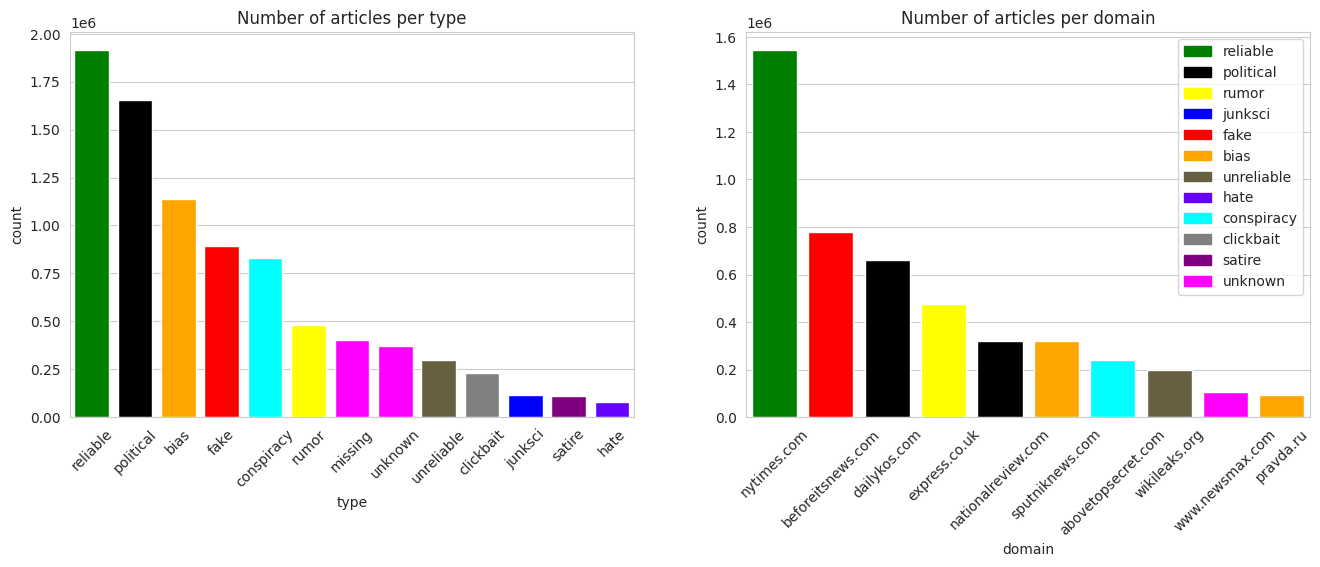
\includegraphics[width=1\textwidth]{combdist}
  \caption{Article type and domain distribution}
  \label{fig:combdist}
\end{figure}
\subsubsection{Vocabulary sizes}
As an exploration, we decided to calculate the vocabulary size of a sample of the dataset. We did this by first
tokenising the sample, and then counting the
unique tokens. We then repeated this process after removing stopwords, and finally after stemming the tokens. The
results are shown in table \ref{tab:vocab_sizes}. As we can see the vocabulary decreases slightly after removing
stopwords, and significantly after stemming. As we see, removing a list of common words doesn't reduce the vocabulary
much, but reducing words to their root does.

\begin{table}[h]
    \centering
    \begin{tabular}{r| c | c | c| c}
      Data& vocabulary size & vocabulary size (lowered) & \% decrease & \% decrease (lowered)\\
        \hline
      Sample data& 21016 & 18011 & 0\% & 0\% \\
    \hline
      Removed stopwords & 20674 & 17865 & 1.63\% & 0.81\% \\
    \hline
      Stemmed & 12654 & 12703 & 39.8\% & 29.5\%
    \end{tabular}
    \caption{Vocabulary sizes}
    \label{tab:vocab_sizes}
\end{table}

% TODO ADD THESE NUMBERS TO TABLE


\subsubsection{Classifying truth per domain}\label{sec:truth_pr_domain}
A central aspect of the dataset, is the way it classifies news articles in terms of reliability. The creators of the
dataset have chosen to classify the articles per domain, meaning that all the articles from any given domain will be
given the same level of credibility.

\subsubsection{Duplicated articles}\label{sec:dup_articles}
Another thing we realised quite quickly, is that the dataset contains a significant amount of duplicated articles as
seen in table \ref{tab:dupart}.

\begin{table}[htpb]
  \centering
  \caption{Duplicated articles and their domain}
  \label{tab:dupart}
  \begin{tabular}{r | c | c| c| c}
      domain & type & content & count&\% of corpus \\ \hline
      nationalreview.com & political & Plus one article on Google Plus (Thanks to al... & 273388 & 3.2\%\\ \hline
      wikileaks.org & unreliable & Tor Tor is an encrypted anonymising network t... & 169259 & 2.0\% \\ \hline
      sputniknews.com & bias & Dear readers, we are excited to announce that ... & 102671 & 1.2\%\\
    \multicolumn{5}{c}{$\vdots$}
  \end{tabular}
\end{table}
As we can see, this is due to different popups that the webscraper has encountered as it
was trying to scrape the dataset. These duplicated articles were simply removed before we trained our model.

\subsubsection{Lower dimensionality}
We have made a 2D UMAP representation of the dataset, which is a form of non-linear dimensionality reduction. We've
trained the model unsupervised to get the inherent distribution of the data without any labelling bias.
\begin{figure}[htpb]
  \centering
  \includegraphics[width=0.8\textwidth]{figures/umapFakeNewsClasses}
  \caption{UMAP representation}
  \label{fig:umap_explore}
\end{figure}

The plot, figure \ref{fig:umap_explore} contains a large cluster which contains a rough mix of everything which UMAP
couldn't separate as well as some more concentrated clusters of junk science and conspiracy articles. On the boundaries
of the big cluster, we have some more concentrated clusters that the model was able to separete, this includes reliable
and fake. Away from the main cluster, we have a large cluster of almost entirely reliable content the model was easily able
to separate. As we see in figure \ref{fig:combdist} NY Times is by far the most represented domain, and all the
articles coming from this domain is marked as reliable. Consequently, the large reliable cluster we see here consists of the
articles from NY Times. We were able to determine this, by querying the UMAP model for the specific coordinates of various articles from a selection of sources. Other clusters far apart include unreliable and rumors.\\
The clear deliniation of the reliable data served as part of our justification for the binary grouping of \textit{reliable} and \textit{unreliable}. 





\section{Data pipeline}
In this section we'll discuss the processing steps we applied to the data, after retrieving it and converting it to a
useful format. This goes in addition to any steps taken in the previous section. 

\subsubsection{What features to focus on}
For the models, we chose to primarily focus on the content of the articles as predictors for whether a given article is
fake or not. Whilst we were tempted to include "domain" initially, after the discovery discussed in section \textbf{REF},
we decided against We also chose to ignore the titles of the articles, as these where often simply reflections of the
content. \todo{Correct?}

\subsubsection{Grouping}
Whilst it is possible to use logistic regression for multi-class classification, we instead chose to build a binary
classifier, that tries to establish wether an article is "reliable" or not. Because of our focus on the reliability of
the article, we chose to encode all "reliable" articles as 1's, whilst the rest of the types ("fake", "bias", etc.) got
encoded as 0's. With this approach we will be (perhaps unfairly) strict in our judgement of a given article, but we
reason that it is better to accidentally label a reliable article as false, than it is to accidentally label a false
article as reliable. \todo{Maybe we should include an appendix with alternative model results for hard classification of
fake news?}

\subsubsection{Splitting the dataset}
At this point we start moving into territory where we need to split our data. So we decided to split our data into into
a training, validation and testing set, with a 80-10-10 split.

\subsubsection{Tokenization}
After filtering out duplicate articles ( \textbf{REFERECE TO PREVIOUS SECTION}), and deciding to focus on the content of
the articles for our input, the next step was to tokenize the data. We tokenized the text by first splitting it into
individual words, removing stop words and using lemmitization to further reduce the vocabulary by condensing words into
base form.

\subsubsection{Feature extraction using TF-IDF}
After treated the content column, we were then able to train a TF-IDF (Term Frequency - Inverse Document Frequency)
model on it. This model looks at how often a given token (word) appears in an article, and compares it to how big that
document is. By training this model, we essentially output a large vector, which we can use to encode the tokens into a
large matrix that can be fed into our models.

\subsubsection{Dimensionality reduction using Truncated Single Value Decomposition (SVD)}
After encoding the data using our TF-IDF model, we were left with quite a large input space, which meant that it would
be useful for us to reduce the dimensionality of our input matrix. In other words, we wanted to group similar elements
(or flags) together, such that the models we build have a more clear delineation between inputs. To this we used
truncated single value decomposition (SVD), that works by factoring a matrix with the hopes to extract most impactful
elements of it.




\section{Simple model: Logistic Regression (1/2 page)} 
For our baseline, we chose to use a logistic regression model. Much of the heavy lifting in developing this model took place in the previous sections,
so once we reached this step we chose to just use a relatively naive implementation, using the default arguments provided
by \textit{scikit-learn}. This meant we had the following hyperparameters for our model. \textbf{Penalty}: l2. This form of penalty adds a penalty that is equal to the square of the magnitude of the
    coefficients of the model. In other words, it tries to limit the influence that any single coefficient has on the
<<<<<<< HEAD
    model. \textbf{Solver}: lbfgs (limited memory BFGS). This solver is one of the most general logistic regression
    solvers, and is therefore a natural fit when we don't wish to direct it further.
=======
    model. \textbf{Solver}: lbfgs (limited memory BFGS). This solver is especially useful on "smaller" datasets (such as
    ours), both because it is quick to train, but also because it is memory efficient which helps us on limited
    hardware. TK REMOVE PRIOR SENTENCE???
>>>>>>> refs/remotes/origin/final_touches


\section{Complex models}
\subsection{XGBoost}
XGBoost is an ensemble learner, meaning it is a collection of smaller models. The way this algorithm is trained, is we start with a decision tree. In every boosting round, which is done 10 times, we find the weights responsible for incorrect classifications, boost them (making them more important for the specific tree), and attempt to minimize the loss. This means every subsequent tree is trying to correct the errors of the previous tree.

\subsection{Large DNN}
This model uses TF-IDF 4096 without further dimensionality reduction. It is a simple feed-forward network with the layers 1024, DO, 512, DO, 256, DO, 128, DO, 64, 1 where DO is a drop-out layer of 0.2, meaning every epoch it resets 20\% of the weights. The idea with this funnel-shaped network was that it would reduce the dimensions on its own and learn how to classify the dataset with minimal loss of data. Shortcomings of the model: The model is on the larger side (57 MB), was slow to train and has a slow inference speed.

\subsection{Small DNN}
This model is a more traditionally shaped feed-forward network. Since the data was passed through dimensionality reduction
already, it means the initial input space can be smaller. The layers are: 384, DO, 512, DO, 512, DO, 128, DO', 16, 1.
DO' is a dropout of 0.1 and DO is the same as in the large DNN.


\section{Results and evaluation}
In this section we will discuss the performance of both our simple and complex models, and discuss how these stack up
against eachother. We will discuss the accuracy and performance on both the FakeNewsCorpus dataset and the LIAR
dataset. And we will end of this evaluation by discussing the challenges in general fake news classifiers, and the
ethical and practical challenges such a model encounters.

\subsection{Relative performance on FakeNewsCorpus}
Let's begin by looking at our models performance on the FakeNewsCorpus dataset. As we see from table \ref{tab:fakenewsperformance},
all of our models performed admirably when being run against the test set, with our more complex models pulling ahead
comfortably.

\begin{table}[htpb]
  \centering
  \caption{Model performance on FakeNewsCorpus dataset}
  \label{tab:fakenewsperformance}

  \begin{tabular}{c|cccc}
    Model & Logistic Regression & Large DNN & Small DNN & XGBoost \\ \hline
    Precision (Reliable / Unreliable) & 0.95 / 0.98 & 0.83 / 0.94 & 0.92 / 0.98 & 0.87 / 0.95 \\ \hline
    Recall (Reliable / Unreliable) & 0.95 / 0.98 & 0.87 / 0.92 & 0.95 / 0.96 & 0.89 / 0.94 \\ \hline
    F1-Score (Reliable / Unreliable) & 0.95 / 0.98 & 0.85 / 0.93 & 0.93 / 0.97 & 0.88 / 0.95 \\ \hline
    Size & 16.6 MB & 121 MB & 34 MB & 29.8 MB 
  \end{tabular}
\end{table}

\subsection{Generalisability and why the models are shit at LIAR}
However, whilst these results are impressive, they also hint that our models might be overfitted to our domain. This is
likely due to the nature of the dataset we used for training not being general enough, which means a broader selection
of data sources and data sets would be needed to achieve a more generalisable model. This issue is highlighted in
particular by the relatively terrible accuracy acheived on the LIAR dataset as seen in table \ref{tab:liarperformance}.

\begin{table}[htpb]
  \centering
  \caption{Model performance on LIAR dataset}
  \label{tab:liarperformance}
  \begin{tabular}{c|cccc}
    Model & Logistic Regression & Large DNN & Small DNN & XGBoost \\ \hline
    Precision (True / False) & 0.17 / 0.84  & 0.18 / 0.84 & 0.18 / 0.84 & 0.17 / 0.84 \\ \hline
    Recall (True / False) & 0.13 / 0.88 & 0.07 / 0.94 & 0.12 / 0.89 & 0.19 / 0.83 \\ \hline
    F1-Score (True / False) & 0.14 / 0.86 & 0.10 / 0.89 & 0.14 / 0.87 & 0.18 / 0.84 \\ \hline
  \end{tabular}
\end{table}

\subsubsection{ROC comparison}
We decided to visualize the performance using ROC comparison, and as we see from figure \ref{fig:roc}, all of the models lose
(almost) all their predictive power when we apply them to the LIAR dataset.

\begin{figure}[htpb]
  \centering
  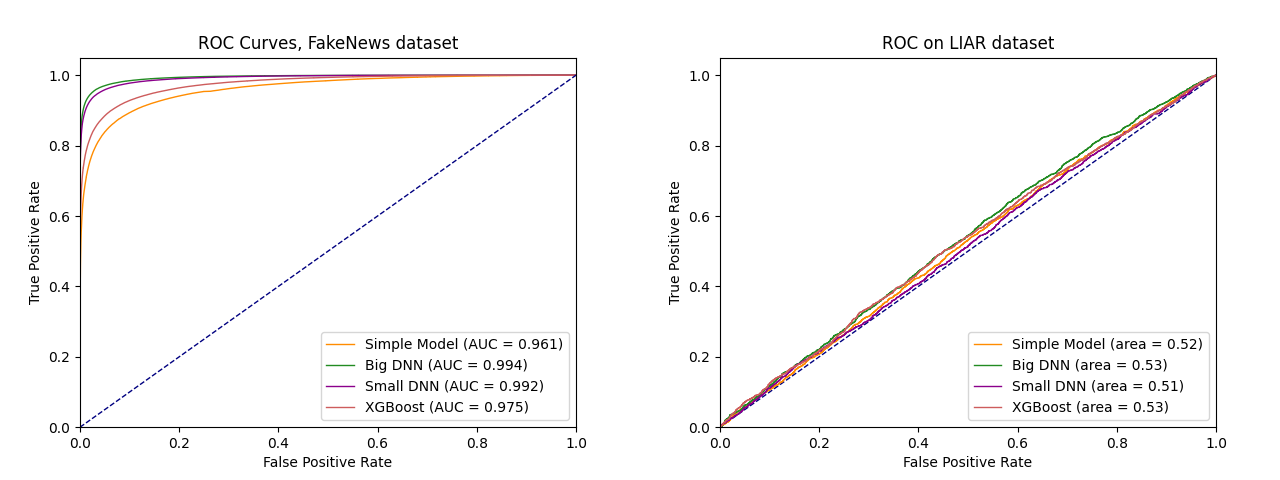
\includegraphics[width=0.8\textwidth]{figures/ROC_combined}
  \caption{ROC comparison - FakeNewsCorpus and LIAR}
  \label{fig:roc}
\end{figure}


\subsubsection{UMAP and lack of seperability in LIAR}
As we did in the beginning, we decided to put the LIAR dataset through the UMAP model that was fitted to the
FakeNewsCorpus dataset. From figure (REF) we see that the articles in the LIAR dataset completely lacks seperability,
meaning our models have no real way of delineating them from eachother.


\subsection{Ethical considerations with fake news classification}
The subpar performance on the LIAR dataset highlights the difficulty in creating a proper fake news classifier. When trying to
generalise a model, questions about what consitutes reliable, fake or misleading news quickly arises. Does a publication raising awareness
of the real side-effects of the HPV vaccine count as reliable? And how does an algorithm distinguish this from a
publication spreading fake statistics of the corona vaccine?. Whilst there are publishers that we all (generally)
accept as being reliable, and others that are generally percieved as being unreliable, the exact line delineating the
two is hard (if not impossible) to strongly define.


\section{Conclusion}

\subsection{Dataset issues}
As has been highlighted throughout this report, the FakeNewsCorpus dataset has many shortcomings, chief among which is
the classification of reliability based on domain. As we see, our classifiers trained on this dataset, generalise quite
poorly outside of their original domain.

\subsection{TF-IDF limitations}
Another key limitation is the use of TF-IDF model for embedding the content. The limitation is that TF-IDF does
not provide us with local context. It instead provides us with a single embedding representing the important keywords of the
entire document, without understanding the semantics of individual sentences. Here, a more complex word embedding model
would be a sensible alternative to try.

\subsection{Ethical considerations with fake news classification}
The subpar performance on the LIAR dataset highlights the difficulty in creating a proper fake news classifier. When trying to
generalise a model, questions about what consitutes reliable, fake or misleading news quickly arises. Does a publication raising awareness
of the real side-effects of the HPV vaccine count as reliable? And how does an algorithm distinguish this from a
publication spreading fake statistics of the corona vaccine?. Whilst there are publishers that we all (generally)
accept as being reliable, and others that are generally percieved as being unreliable, the exact line delineating the
two is hard (if not impossible) to strongly define.


In this technical report we described the exploration of three different models for fake news classification. We started
by outlining the data import, exploration and processing we applied to the FakeNewsCorpus dataset. The processing
included both tokenisation, feature extracting using TF-IDF and dimensionality reduction through single value
decomposition. We build a logistic regression model to serve as our baseline, and then constructed three more complex
models (two DNNs and an XGBoost model). Whilst all of the models performed admirably on the FakeNewsCorpus dataset, they
all failed to generalise when we tested them against another dataset (LIAR). As discussed in our evaluation section,
this is likely due both to the quality of our dataset and the inherent difficulties in constructing fake news
classifiers in general. In the end we conclude that our approach has failed to build a general fake news classifier, and
that more sophisticated tools need to be incorporated in order to achieve generalisable success.





% \subsection{Citations}
% Citations use \verb+natbib+. The documentation may be found at
% \begin{center}
%\url{http://mirrors.ctan.org/macros/latex/contrib/natbib/natnotes.pdf}
% \end{center}

%Here is an example usage of the two main commands (\verb+citet+ and \verb+citep+): Some people thought a thing \citep{kour2014real, hadash2018estimate} but other people thought something else \citep{kour2014fast}. Many people have speculated that if we knew exactly why \citet{kour2014fast} thought this\dots

%\subsection{Figures}
%\lipsum[10]
%See Figure \ref{fig:fig1}. Here is how you add footnotes. \footnote{Sample of the first footnote.}
%\lipsum[11]
%
%\begin{figure}
%	\centering
%	\fbox{\rule[-.5cm]{4cm}{4cm} \rule[-.5cm]{4cm}{0cm}}
%	\caption{Sample figure caption.}
%	\label{fig:fig1}
%\end{figure}
%
%\subsection{Tables}
%See awesome Table~\ref{tab:table}.
%
%The documentation for \verb+booktabs+ (`Publication quality tables in LaTeX') is available from:
%% \begin{center}
%	% \url{https://www.ctan.org/pkg/booktabs}
%% \end{center}
%
%
%\begin{table}
%	\caption{Sample table title}
%	\centering
%	\begin{tabular}{lll}
%		\toprule
%		\multicolumn{2}{c}{Part}                   \\
%		\cmidrule(r){1-2}
%		Name     & Description     & Size ($\mu$m) \\
%		\midrule
%		Dendrite & Input terminal  & $\sim$100     \\
%		Axon     & Output terminal & $\sim$10      \\
%		Soma     & Cell body       & up to $10^6$  \\
%		\bottomrule
%	\end{tabular}
%	\label{tab:table}
%\end{table}
%
%\subsection{Lists}
%\begin{itemize}
%	\item Lorem ipsum dolor sit amet
%	\item consectetur adipiscing elit.
%	\item Aliquam dignissim blandit est, in dictum tortor gravida eget. In ac rutrum magna.
%\end{itemize}
%
%%%% Uncomment this section and comment out the \bibliography{references} line above to use inline references.
%\bibliographystyle{unsrtnat}
%\bibliography{references}  %%% Uncomment this line and comment out the ``thebibliography'' section below to use the external .bib file (using bibtex) .
%
%
%%%% Uncomment this section and comment out the \bibliography{references} line above to use inline references.
%% \begin{thebibliography}{1}
%
%% 	\bibitem{kour2014real}
%% 	George Kour and Raid Saabne.
%% 	\newblock Real-time segmentation of on-line handwritten arabic script.
%% 	\newblock In {\em Frontiers in Handwriting Recognition (ICFHR), 2014 14th
%% 			International Conference on}, pages 417--422. IEEE, 2014.
%
%% 	\bibitem{kour2014fast}
%% 	George Kour and Raid Saabne.
%% 	\newblock Fast classification of handwritten on-line arabic characters.
%% 	\newblock In {\em Soft Computing and Pattern Recognition (SoCPaR), 2014 6th
%% 			International Conference of}, pages 312--318. IEEE, 2014.
%
%% 	\bibitem{hadash2018estimate}
%% 	Guy Hadash, Einat Kermany, Boaz Carmeli, Ofer Lavi, George Kour, and Alon
%% 	Jacovi.
%% 	\newblock Estimate and replace: A novel approach to integrating deep neural
%% 	networks with existing applications.
%% 	\newblock {\em arXiv preprint arXiv:1804.09028}, 2018.
%
%% \end{thebibliography}
%

\end{document}
